% Options for packages loaded elsewhere
\PassOptionsToPackage{unicode}{hyperref}
\PassOptionsToPackage{hyphens}{url}
%
\documentclass[
]{article}
\usepackage{amsmath,amssymb}
\usepackage{lmodern}
\usepackage{ifxetex,ifluatex}
\ifnum 0\ifxetex 1\fi\ifluatex 1\fi=0 % if pdftex
  \usepackage[T1]{fontenc}
  \usepackage[utf8]{inputenc}
  \usepackage{textcomp} % provide euro and other symbols
\else % if luatex or xetex
  \usepackage{unicode-math}
  \defaultfontfeatures{Scale=MatchLowercase}
  \defaultfontfeatures[\rmfamily]{Ligatures=TeX,Scale=1}
\fi
% Use upquote if available, for straight quotes in verbatim environments
\IfFileExists{upquote.sty}{\usepackage{upquote}}{}
\IfFileExists{microtype.sty}{% use microtype if available
  \usepackage[]{microtype}
  \UseMicrotypeSet[protrusion]{basicmath} % disable protrusion for tt fonts
}{}
\makeatletter
\@ifundefined{KOMAClassName}{% if non-KOMA class
  \IfFileExists{parskip.sty}{%
    \usepackage{parskip}
  }{% else
    \setlength{\parindent}{0pt}
    \setlength{\parskip}{6pt plus 2pt minus 1pt}}
}{% if KOMA class
  \KOMAoptions{parskip=half}}
\makeatother
\usepackage{xcolor}
\IfFileExists{xurl.sty}{\usepackage{xurl}}{} % add URL line breaks if available
\IfFileExists{bookmark.sty}{\usepackage{bookmark}}{\usepackage{hyperref}}
\hypersetup{
  pdftitle={Assignment 3: Predators, Prey, and Foodwebs},
  hidelinks,
  pdfcreator={LaTeX via pandoc}}
\urlstyle{same} % disable monospaced font for URLs
\usepackage[margin=1in]{geometry}
\usepackage{color}
\usepackage{fancyvrb}
\newcommand{\VerbBar}{|}
\newcommand{\VERB}{\Verb[commandchars=\\\{\}]}
\DefineVerbatimEnvironment{Highlighting}{Verbatim}{commandchars=\\\{\}}
% Add ',fontsize=\small' for more characters per line
\usepackage{framed}
\definecolor{shadecolor}{RGB}{248,248,248}
\newenvironment{Shaded}{\begin{snugshade}}{\end{snugshade}}
\newcommand{\AlertTok}[1]{\textcolor[rgb]{0.94,0.16,0.16}{#1}}
\newcommand{\AnnotationTok}[1]{\textcolor[rgb]{0.56,0.35,0.01}{\textbf{\textit{#1}}}}
\newcommand{\AttributeTok}[1]{\textcolor[rgb]{0.77,0.63,0.00}{#1}}
\newcommand{\BaseNTok}[1]{\textcolor[rgb]{0.00,0.00,0.81}{#1}}
\newcommand{\BuiltInTok}[1]{#1}
\newcommand{\CharTok}[1]{\textcolor[rgb]{0.31,0.60,0.02}{#1}}
\newcommand{\CommentTok}[1]{\textcolor[rgb]{0.56,0.35,0.01}{\textit{#1}}}
\newcommand{\CommentVarTok}[1]{\textcolor[rgb]{0.56,0.35,0.01}{\textbf{\textit{#1}}}}
\newcommand{\ConstantTok}[1]{\textcolor[rgb]{0.00,0.00,0.00}{#1}}
\newcommand{\ControlFlowTok}[1]{\textcolor[rgb]{0.13,0.29,0.53}{\textbf{#1}}}
\newcommand{\DataTypeTok}[1]{\textcolor[rgb]{0.13,0.29,0.53}{#1}}
\newcommand{\DecValTok}[1]{\textcolor[rgb]{0.00,0.00,0.81}{#1}}
\newcommand{\DocumentationTok}[1]{\textcolor[rgb]{0.56,0.35,0.01}{\textbf{\textit{#1}}}}
\newcommand{\ErrorTok}[1]{\textcolor[rgb]{0.64,0.00,0.00}{\textbf{#1}}}
\newcommand{\ExtensionTok}[1]{#1}
\newcommand{\FloatTok}[1]{\textcolor[rgb]{0.00,0.00,0.81}{#1}}
\newcommand{\FunctionTok}[1]{\textcolor[rgb]{0.00,0.00,0.00}{#1}}
\newcommand{\ImportTok}[1]{#1}
\newcommand{\InformationTok}[1]{\textcolor[rgb]{0.56,0.35,0.01}{\textbf{\textit{#1}}}}
\newcommand{\KeywordTok}[1]{\textcolor[rgb]{0.13,0.29,0.53}{\textbf{#1}}}
\newcommand{\NormalTok}[1]{#1}
\newcommand{\OperatorTok}[1]{\textcolor[rgb]{0.81,0.36,0.00}{\textbf{#1}}}
\newcommand{\OtherTok}[1]{\textcolor[rgb]{0.56,0.35,0.01}{#1}}
\newcommand{\PreprocessorTok}[1]{\textcolor[rgb]{0.56,0.35,0.01}{\textit{#1}}}
\newcommand{\RegionMarkerTok}[1]{#1}
\newcommand{\SpecialCharTok}[1]{\textcolor[rgb]{0.00,0.00,0.00}{#1}}
\newcommand{\SpecialStringTok}[1]{\textcolor[rgb]{0.31,0.60,0.02}{#1}}
\newcommand{\StringTok}[1]{\textcolor[rgb]{0.31,0.60,0.02}{#1}}
\newcommand{\VariableTok}[1]{\textcolor[rgb]{0.00,0.00,0.00}{#1}}
\newcommand{\VerbatimStringTok}[1]{\textcolor[rgb]{0.31,0.60,0.02}{#1}}
\newcommand{\WarningTok}[1]{\textcolor[rgb]{0.56,0.35,0.01}{\textbf{\textit{#1}}}}
\usepackage{graphicx}
\makeatletter
\def\maxwidth{\ifdim\Gin@nat@width>\linewidth\linewidth\else\Gin@nat@width\fi}
\def\maxheight{\ifdim\Gin@nat@height>\textheight\textheight\else\Gin@nat@height\fi}
\makeatother
% Scale images if necessary, so that they will not overflow the page
% margins by default, and it is still possible to overwrite the defaults
% using explicit options in \includegraphics[width, height, ...]{}
\setkeys{Gin}{width=\maxwidth,height=\maxheight,keepaspectratio}
% Set default figure placement to htbp
\makeatletter
\def\fps@figure{htbp}
\makeatother
\setlength{\emergencystretch}{3em} % prevent overfull lines
\providecommand{\tightlist}{%
  \setlength{\itemsep}{0pt}\setlength{\parskip}{0pt}}
\setcounter{secnumdepth}{-\maxdimen} % remove section numbering
\ifluatex
  \usepackage{selnolig}  % disable illegal ligatures
\fi

\title{Assignment 3: Predators, Prey, and Foodwebs}
\author{}
\date{\vspace{-2.5em}}

\begin{document}
\maketitle

\hypertarget{community-stability-connections-count}{%
\subsection{1. Community Stability: connections
count}\label{community-stability-connections-count}}

With \(S=250,\sigma=0.3\), how does stability depend on \(C\)?

\begin{Shaded}
\begin{Highlighting}[]
\FunctionTok{library}\NormalTok{(ggplot2)}
\end{Highlighting}
\end{Shaded}

\begin{verbatim}
## Warning in register(): Can't find generic `scale_type` in package ggplot2 to
## register S3 method.
\end{verbatim}

\begin{Shaded}
\begin{Highlighting}[]
\FunctionTok{library}\NormalTok{(psych)}
\end{Highlighting}
\end{Shaded}

\begin{verbatim}
## 
## Attaching package: 'psych'
\end{verbatim}

\begin{verbatim}
## The following objects are masked from 'package:ggplot2':
## 
##     %+%, alpha
\end{verbatim}

\begin{Shaded}
\begin{Highlighting}[]
\NormalTok{S }\OtherTok{\textless{}{-}} \DecValTok{250}
\NormalTok{sigma }\OtherTok{\textless{}{-}} \FloatTok{0.3}

\NormalTok{MayMatrix}\OtherTok{\textless{}{-}}\ControlFlowTok{function}\NormalTok{(S,C,sigma)\{}
  \DocumentationTok{\#\# This matrix determines the connections}
\NormalTok{  A}\OtherTok{\textless{}{-}}\FunctionTok{matrix}\NormalTok{(}\FunctionTok{runif}\NormalTok{(S}\SpecialCharTok{*}\NormalTok{S),S,S)}
  \DocumentationTok{\#\# Contains the values for the connections}
\NormalTok{  B}\OtherTok{\textless{}{-}}\FunctionTok{matrix}\NormalTok{(}\FunctionTok{rnorm}\NormalTok{(S}\SpecialCharTok{*}\NormalTok{S,}\FloatTok{0.0}\NormalTok{,sigma),S,S)}
\NormalTok{  A}\OtherTok{\textless{}{-}}\NormalTok{(A}\SpecialCharTok{\textless{}=}\NormalTok{ C)}\SpecialCharTok{*}\DecValTok{1} \CommentTok{\# A matrix contains 1 when A[i,j] \textless{}= C}
\NormalTok{  M}\OtherTok{\textless{}{-}}\NormalTok{A}\SpecialCharTok{*}\NormalTok{B}
  \FunctionTok{diag}\NormalTok{(M)}\OtherTok{\textless{}{-}} \SpecialCharTok{{-}}\DecValTok{1}
  \FunctionTok{return}\NormalTok{(M)}
\NormalTok{\}}

\NormalTok{PPMatrix}\OtherTok{\textless{}{-}}\ControlFlowTok{function}\NormalTok{(S,C,sigma)\{}
  \DocumentationTok{\#\# Determine the signs for the connections}
\NormalTok{  MyS}\OtherTok{\textless{}{-}}\FunctionTok{sign}\NormalTok{(}\FunctionTok{rnorm}\NormalTok{(S}\SpecialCharTok{*}\NormalTok{(S}\DecValTok{{-}1}\NormalTok{)}\SpecialCharTok{/}\DecValTok{2}\NormalTok{))}
\NormalTok{  A}\OtherTok{\textless{}{-}}\FunctionTok{matrix}\NormalTok{(}\DecValTok{0}\NormalTok{,S,S)}
\NormalTok{  A[}\FunctionTok{upper.tri}\NormalTok{(A,}\AttributeTok{diag=}\NormalTok{F)]}\OtherTok{\textless{}{-}}\NormalTok{MyS}
\NormalTok{  D}\OtherTok{\textless{}{-}}\FunctionTok{matrix}\NormalTok{(}\FunctionTok{runif}\NormalTok{(S}\SpecialCharTok{*}\NormalTok{S),S,S)}
\NormalTok{  D}\OtherTok{\textless{}{-}}\NormalTok{(D }\SpecialCharTok{\textless{}=}\NormalTok{ C)}\SpecialCharTok{*}\DecValTok{1}
\NormalTok{  A}\OtherTok{\textless{}{-}}\NormalTok{D}\SpecialCharTok{*}\NormalTok{A}
\NormalTok{  A}\OtherTok{\textless{}{-}}\NormalTok{ A}\SpecialCharTok{{-}}\FunctionTok{t}\NormalTok{(A)}
  \DocumentationTok{\#\# Contains the  values for the connections}
\NormalTok{  B}\OtherTok{\textless{}{-}}\FunctionTok{matrix}\NormalTok{(}\FunctionTok{abs}\NormalTok{(}\FunctionTok{rnorm}\NormalTok{(S}\SpecialCharTok{*}\NormalTok{S,}\FloatTok{0.0}\NormalTok{,sigma)),S,S)}
\NormalTok{  M}\OtherTok{\textless{}{-}}\NormalTok{A}\SpecialCharTok{*}\NormalTok{B}
  \FunctionTok{diag}\NormalTok{(M)}\OtherTok{\textless{}{-}} \SpecialCharTok{{-}}\DecValTok{1}
  \FunctionTok{return}\NormalTok{(M)}
\NormalTok{\}}

\NormalTok{stableQ}\OtherTok{\textless{}{-}} \ControlFlowTok{function}\NormalTok{(m)\{}
  \ControlFlowTok{if}\NormalTok{(}\FunctionTok{tr}\NormalTok{(m)}\SpecialCharTok{\textless{}}\DecValTok{0} \SpecialCharTok{\&} \FunctionTok{det}\NormalTok{(m)}\SpecialCharTok{\textgreater{}}\DecValTok{0}\NormalTok{)\{}
    \FunctionTok{return}\NormalTok{(}\DecValTok{1}\NormalTok{)}
\NormalTok{  \}}\ControlFlowTok{else}\NormalTok{\{}
    \FunctionTok{return}\NormalTok{(}\DecValTok{0}\NormalTok{)}
\NormalTok{  \}}
\NormalTok{\}}


\NormalTok{C }\OtherTok{\textless{}{-}}\FunctionTok{seq}\NormalTok{(}\FloatTok{0.01}\NormalTok{,}\FloatTok{0.5}\NormalTok{,}\AttributeTok{by=}\FloatTok{0.01}\NormalTok{)}

\NormalTok{mays }\OtherTok{\textless{}{-}} \FunctionTok{c}\NormalTok{()}
\ControlFlowTok{for}\NormalTok{ (cs }\ControlFlowTok{in}\NormalTok{ C)\{}
\NormalTok{  mays }\OtherTok{\textless{}{-}} \FunctionTok{append}\NormalTok{(mays,}\FunctionTok{sum}\NormalTok{(}\FunctionTok{replicate}\NormalTok{(}\DecValTok{100}\NormalTok{, }\FunctionTok{stableQ}\NormalTok{(}\FunctionTok{MayMatrix}\NormalTok{(S,cs,sigma)), }\AttributeTok{simplify =} \ConstantTok{TRUE}\NormalTok{ )))}
\NormalTok{\}}
     
\NormalTok{pred }\OtherTok{\textless{}{-}} \FunctionTok{c}\NormalTok{()}
\ControlFlowTok{for}\NormalTok{ (cs }\ControlFlowTok{in}\NormalTok{ C)\{}
\NormalTok{  pred }\OtherTok{\textless{}{-}} \FunctionTok{append}\NormalTok{(pred,}\FunctionTok{sum}\NormalTok{(}\FunctionTok{replicate}\NormalTok{(}\DecValTok{100}\NormalTok{, }\FunctionTok{stableQ}\NormalTok{(}\FunctionTok{PPMatrix}\NormalTok{(S,cs,sigma)), }\AttributeTok{simplify =} \ConstantTok{TRUE}\NormalTok{ )))}
\NormalTok{\}}

\NormalTok{mays }\OtherTok{\textless{}{-}}\NormalTok{ mays}\SpecialCharTok{/}\DecValTok{100}
\NormalTok{pred }\OtherTok{\textless{}{-}}\NormalTok{ pred}\SpecialCharTok{/}\DecValTok{100}


\NormalTok{df}\OtherTok{=}\FunctionTok{data.frame}\NormalTok{(}\AttributeTok{C =}\NormalTok{ C,}
              \AttributeTok{values=}\FunctionTok{c}\NormalTok{(mays, pred),}
              \AttributeTok{matrix=}\FunctionTok{c}\NormalTok{(}\FunctionTok{rep}\NormalTok{(}\StringTok{"May"}\NormalTok{,}\DecValTok{50}\NormalTok{),}\FunctionTok{rep}\NormalTok{(}\StringTok{"Predator{-}Prey"}\NormalTok{,}\DecValTok{50}\NormalTok{))}
\NormalTok{)}


\FunctionTok{ggplot}\NormalTok{(df,}\FunctionTok{aes}\NormalTok{(C,values,}\AttributeTok{col=}\NormalTok{matrix))}\SpecialCharTok{+}\FunctionTok{geom\_line}\NormalTok{() }\SpecialCharTok{+}
  \FunctionTok{ylab}\NormalTok{(}\StringTok{"fraction of stable communities"}\NormalTok{)}
\end{Highlighting}
\end{Shaded}

\includegraphics{Assignment-3_files/figure-latex/question1-1.pdf} We can
see in the plot that both methods of generating matrices result in high
stability for low values of C. The threshold May proves in his paper
\(\sqrt{SC}>\frac{1}{\sigma}\), is \(C>2/45(\approx0.04444)\) when
\(S=250\) and \(\sigma=0.3\). This is consistent with what we simulated.
We can see the predator-prey matrix undergoes a similar transition at a
much higher value of \(C\), closer to 0.25.

\hypertarget{examples-of-particular-dynamics}{%
\subsection{2. Examples of particular
dynamics}\label{examples-of-particular-dynamics}}

\hypertarget{damped-oscillations-of-a-population-to-a-stable-equilibrium-point}{%
\subsubsection{2.1 damped oscillations of a population to a stable
equilibrium
point}\label{damped-oscillations-of-a-population-to-a-stable-equilibrium-point}}

An example system that will show damped oscillations to a stable
equilibrium is the predator-prey model with logistic growth described by
the set of equations. \[
\begin{cases}
\frac{dX}{dt}=(b-d)X(1-X/K)-\alpha XY\\
\frac{dY}{dt}=\alpha\epsilon XY- mY
\end{cases}
\] In general, this system will be stable when the the Jacobian matrix
takes the form \[
A=\begin{bmatrix}
-a & -b\\
c & 0
\end{bmatrix}
\] First we find a feasible equilibirum for the system: \[
\frac{dY}{dt}=0=\alpha\epsilon XY- mY\\
\rightarrow X^*=\frac{m}{\epsilon\alpha}
\] and \[
\frac{dX}{dt}=0=(b-d)X(1-X/K)-\alpha XY \\
\rightarrow Y^*=\frac{b-d}{\alpha}(1-\frac{X}{K})\\
\rightarrow Y^*= \frac{(K\epsilon\alpha-m)(b-d)}{\epsilon\alpha^2K}
\] Then we find the Jacobian matrix at this feasible equilibrium \[
J_{xx}= \frac{\partial}{\partial X}(b-d)X(1-\frac{X}{K}-\alpha XY)\\
= \frac{-2(b-d)X^*}{K}+(b-d)-\alpha Y^*\\
\rightarrow a_{xx}=J_{xx}|_{X^*,Y^*}=\frac{-(b-d)m}{K\epsilon\alpha}\\
\] \(J_{xx}\) is negative whenever \(b>d\) and all constants are
positive. \[
J_{xy}=-\alpha X^*\\
\rightarrow a_{xy}=J_{xy}|_{x^*,Y^*}=-\frac{m}{\epsilon}
\] Again, \(J_{xy}\) is negative whenever \(m>0\)and \(\epsilon>0\). \[
J_{yx}=\alpha\epsilon Y^*\\
\rightarrow a_{yx}=J_{yx}|_{X^*,Y^*}= \frac{(b-d)(K\epsilon\alpha-m)}{\alpha K}
\] This is positive because \(Y^*\) has to be positive. Last we we need
to show that \(a_{yy}=0\) \[
J_{yy}=\alpha\epsilon X^*-m\\
\rightarrow a_{yy}=J_{yy}|_{X^*,Y^*}=\alpha\epsilon \frac{m}{\alpha\epsilon}-m=0
\] Thus \[ 
J= \begin{bmatrix}\frac{-(b-d)m}{K\epsilon\alpha} & -\frac{m}{\epsilon}\\-\frac{(b-d)(K\epsilon\alpha-m)}{\alpha K} & 0\end{bmatrix}
\] at the the feasible equilibrium whenever all constants, and
populations are positive and \(b>d\).

For example, Figure 1 shows the isoclines of this system when the birth
rate of the prey \(b=2\), the death rate of the prey \(d=0.5\), the prey
carrying capacity \(K=15\), , the encounter rate \(\alpha=0.5\), the
conversion efficiency of the predator \(\epsilon=0.9\), and the death
rate for the predator \(m=0.6\). We can see in this plot that whenever
the system starts with \(X>0\) and \(Y>0\), we expect a spiral to the
equilibrium. For example, let's start with \(X=10\) and \(Y=10\). The
resulting oscillation can be seen in figure 2.

\begin{figure}
\centering
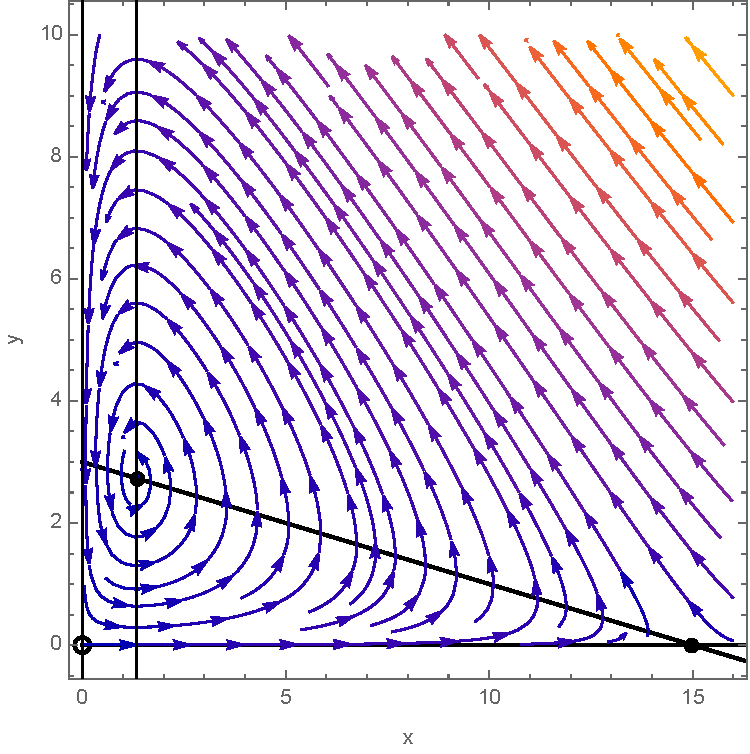
\includegraphics{/Users/katjad/Documents/UChicago/Theoretical Ecology/TheoreticalEcologyCourseGithub/Assignment 3/2Example1}
\caption{The dynamics of the predator prey model with logistic growth}
\end{figure}

\begin{figure}
\centering
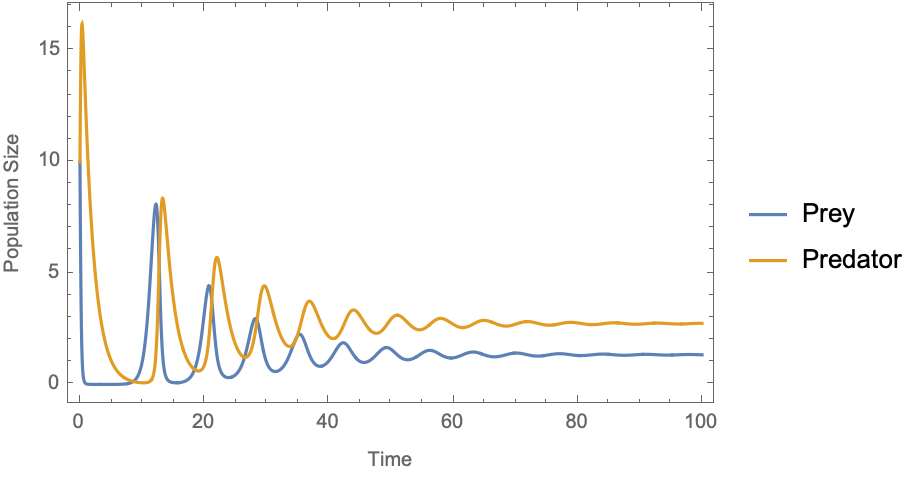
\includegraphics{/Users/katjad/Documents/UChicago/Theoretical Ecology/TheoreticalEcologyCourseGithub/Assignment 3/2Example1Oscillations}
\caption{The dynamics of the predator prey model with logistic growth}
\end{figure}

\hypertarget{stable-cycles}{%
\subsubsection{2.2 stable cycles}\label{stable-cycles}}

The most famous example is the simple Lotka-Volterra model we started
with described by the following system of equations: \[
\begin{cases}
\frac{dN}{dt}=N(a-bP)\\
\frac{dP}{dt}=P(cN-d)
\end{cases}
\] Here \(a\) is the growth rate of the prey \(N\) independent of the
predator \(P\) (this means exponential growth without the predator).
\(b\) is the predation rate of the prey by the predator, \(c\) is the
conversion rate of eaten prey into predator (this is \(b*\epsilon=c\),
where \(\epsilon\) is the conversion efficiency of killed prey into
predator). Lastly, \(d\) is the death rate of the predator without any
prey. We can non-dimensionalize using \[
\begin{cases}
u(\tau)=\frac{cN(t)}{d}\\
v(\tau)=\frac{bP(t)}{a}\\
\tau=at\\
\alpha=\frac{d}{a}
\end{cases}
\] and get \[
\begin{cases}
\frac{du}{d\tau}=u(1-v)\\
\frac{dv}{d\tau}=\alpha v(u-1)
\end{cases}
\]

Again, we start by finding the feasible equilibrium where
\(\frac{du}{d\tau}=0\) and \(\frac{dv}{d\tau}=0\): \[
\begin{cases}
0=u(1-v)\\
0=\alpha v(u-1)
\end{cases}\\
\rightarrow \begin{cases}
u^*=1\\
v^*=1
\end{cases}
\] The Jacobian matrix at this feasible equilibrium is \[
J=
\begin{bmatrix}
1-v & -u\\
\alpha v & \alpha u-\alpha
\end{bmatrix}\\
A=J|_{u=u^*,v=v^*}=
\begin{bmatrix}
0 & -1\\
\alpha & 0
\end{bmatrix}
\] Here, \(Tr(A)=0,Det(A)>0\) so we know there is a fixed point center
and thus oscillations are stable with the magnitude determined by the
constants.

Figure 3 shows the isoclines and figure 4 the dynamics of this system
when \(a=2, b=1, c=0.9, d=0.5, N[0]=5, P[0]=2\)

\begin{figure}
\centering
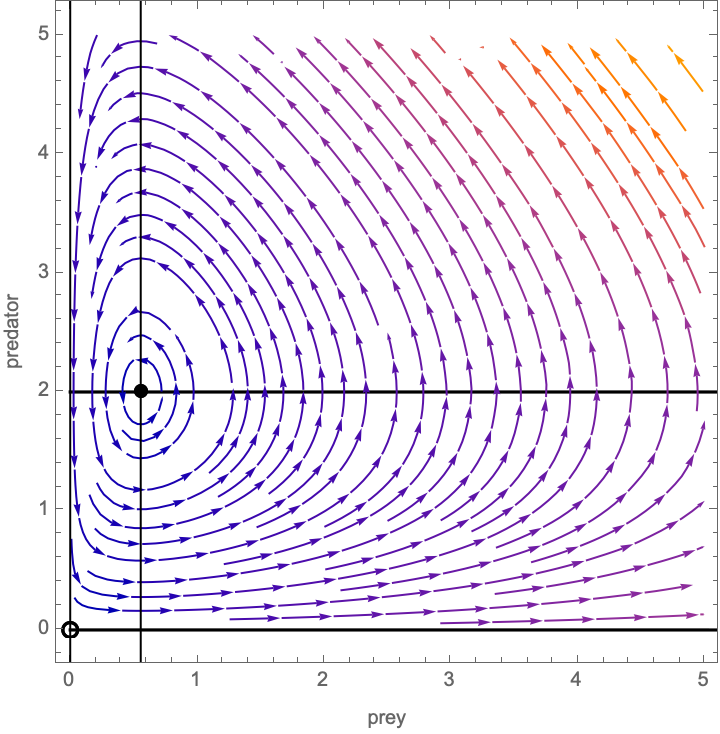
\includegraphics{/Users/katjad/Documents/UChicago/Theoretical Ecology/TheoreticalEcologyCourseGithub/Assignment 3/2Example2}
\caption{The dynamics and isoclines of the basic, Lotka-Volterra
predator-prey model}
\end{figure}

\begin{figure}
\centering
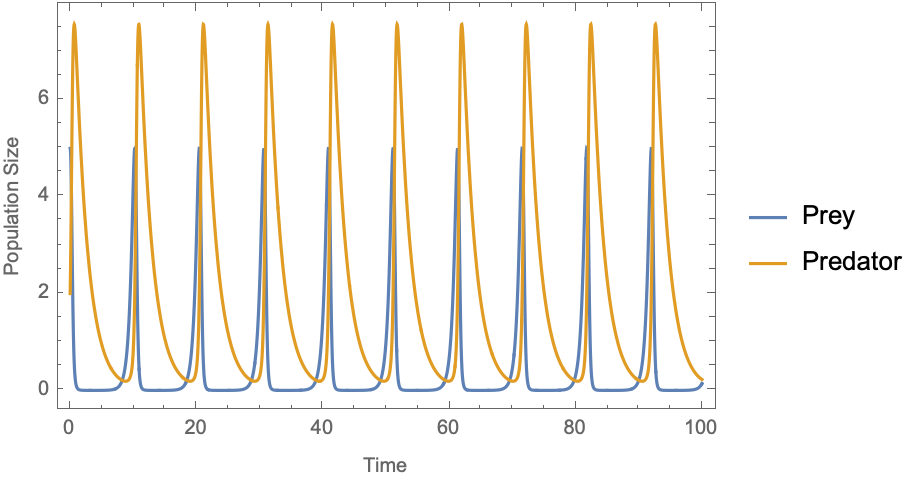
\includegraphics{/Users/katjad/Documents/UChicago/Theoretical Ecology/TheoreticalEcologyCourseGithub/Assignment 3/2Example2StableOscillations}
\caption{The dynamics of the basic, Lotka-Volterra predator-prey model}
\end{figure}

\hypertarget{unstable-dynamics-away-from-a-nontrivial-equilibrium}{%
\subsubsection{2.3 unstable dynamics away from a nontrivial
equilibrium}\label{unstable-dynamics-away-from-a-nontrivial-equilibrium}}

An example of a model where we get an unstable nontrivial equilibrium is
two consumers competing for the same resource where the intraspecific
competition is larger than the interspecific competition. This can be
described by the system: \[
\begin{cases}
\frac{dN_1}{dt}=N_1(r_1-\alpha_{11}N_1-\alpha_{12}N_2)\\
\frac{dN_2}{dt}=N_2(r_2-\alpha_{22}N_2-\alpha_{21}N_1)
\end{cases}
\] \(N_1\) and \(N_2\) are the competitors, \(r_1\) and \(r_2\) their
growth rates, \(\alpha_{11}\) and \(\alpha_{22}\) the strength of their
intraspecific competition and \(\alpha_{12}\) and \(\alpha_{21}\) the
strength of interspecific competition of species 2 on species 1 and
species 1 on species 2 respectively.

We can solve for the equilibria and get four equilibria of which only
the fourth is non-trivial. \[ 
\begin{cases} N_1^*=0\\ N_2^*=0\end{cases}
\begin{cases} N_1^*=0\\ N_2^*=-\frac{r_2}{a_{22}}\end{cases}
\begin{cases} N_1^*=\frac{r_1}{a_{11}}\\ N_2^*=0\end{cases}
\begin{cases} N_1^*=-\frac{a_{22}r_1-a_{12}r_2}{a_{12}a{21}-a_{11}a_{22}}\\ N_2^*=-\frac{-a_{21}r_1+a_{11}r_2}{a_{12}a_{21}-a_{11}a_{22}}\end{cases}
\] We can then look at the Jacobian to determine the conditions for the
feasible equilibrium to be unstable. To simplify, we will take the
Jacobian of the per capita growth rates of both species. \[
J= 
\begin{bmatrix}
-\alpha_{11} & -\alpha_{12}\\
-\alpha_{21} & -\alpha_{22}
\end{bmatrix}
\] For this system to be stable, the real parts of the eigenvalues needs
to be negative. The eigenvalues are \[
\lambda_1=\frac{-\alpha_{11}-\alpha_{22}+\sqrt{\alpha_{11}^2-2\alpha_{11}\alpha_{22}+\alpha_{22}^2+4\alpha_{12}\alpha_{21}}}{2}\\
\lambda_2=\frac{-\alpha_{11}-\alpha_{22}-\sqrt{\alpha_{11}^2-2\alpha_{11}\alpha_{22}+\alpha_{22}^2+4\alpha_{12}\alpha_{21}}}{2}
\] Thus, the system is unstable whenever
\(\alpha_{11}\alpha_{22}<\alpha_{12}\alpha_{21}\).

For example, let \(r_1=r_2=2\), \(\alpha_{11}=0.5\), \(alpha_{12}=0.7\),
\(\alpha_{22}=0.6\), and \(\alpha_{21}=0.8\). The resulting stream plot
shows an unstable equilibrium and no matter how close to this
equilibirum the population starts, it will converge to one of the
single-species equilibria.

\begin{figure}
\centering
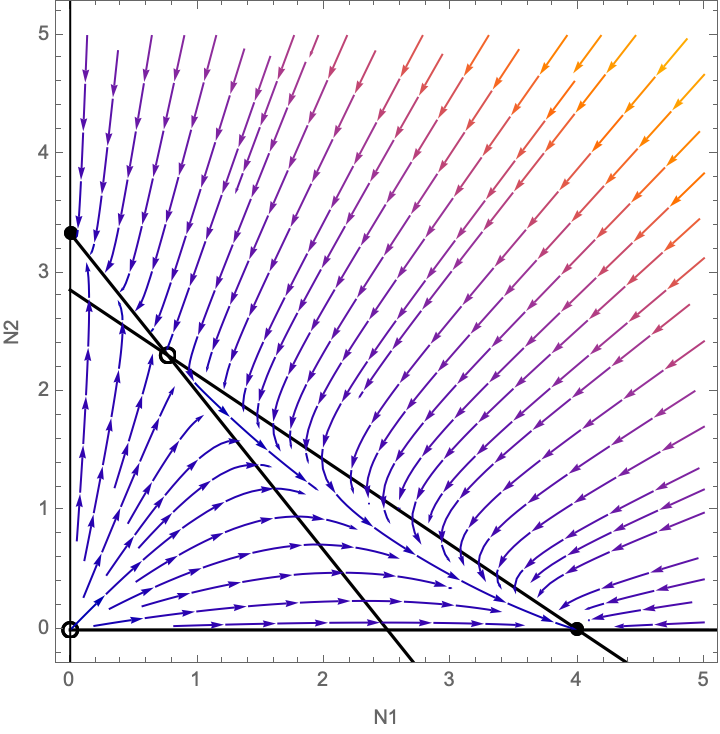
\includegraphics{/Users/katjad/Documents/UChicago/Theoretical Ecology/TheoreticalEcologyCourseGithub/Assignment 3/2Example3}
\caption{The dynamics of the competition model}
\end{figure}

\hypertarget{chaotic-dynamics}{%
\subsubsection{2.4 chaotic dynamics}\label{chaotic-dynamics}}

The probably most famous example of a simple equation leading to chaotic
behavior is Robert May's logistic map model of population dynamics in a
single species \(x\).

\[
x_{n+1}=rx_n(1-x_n)
\] Once again, \(r\) represents a growth rate for the population but
this time \(x\) is not the absolute population size but rather a
fraction representing the proportion of the maximum (carrying capacity)
population size possible.

Again we find candidates for stability, where \(x_{n+1}=x_n=x^*\). This
is the case when \(x^*_1=0\) or \(x^*_2=1-\frac{1}{r}\) (only feasible
equilibirum).

We take the derivative to test for stability at the feasible
equilibirum. \[
f'(x)=\frac{d}{dx}rx(1-x)=r(1-x)\\
f'(x)|_{x^*_2}=r(1-2(1-\frac{1}{r}))=2-r
\] If \(|2-r|<1\), the point is stable, so for \(1<r<3\). Next, we look
at the period-2 stable points, where
\(x_{n+2}=f(x_{n+1})=f(f(x_n))=f^{(2)}(x_n)\). \[ 
x= f(f(x))= rf(x)(1-f(x))\\=r^2x(1-x)(1-rx(1-x))\\=-r^2x(x-1)(rx^2-rx+1)
\] There are three solutions for which \(x>0\) \(x=1-\frac{1}{r}\) This
is the same we found for the stable equilibirum case and we know it is
unstable for \(r>3\). The other two solutions are more difficult to
predict the behavior for \[
x=\frac{r+1\pm\sqrt(r^2-2r-3)}{2r}=y_{1,2}
\] We need to look at
\(|\frac{\partial}{\partialx}f^{(2)}(x)|y_1<1\).This eventually will
give us another value range similar to \(1<r<3\) for which there is a
stable 2-period solution. Then we repeat the same for period-4,
period-8, etc. All of them will occupy smaller and smaller ranges of
\(r\) approaching 3.57, after which the dynamics are chaotic.

To summarize for low values of \(r\), the dynamics are stable, for
intermediate values we get oscillations of different periods, but for
values of \(r\) close to 4, the dynamics become chaotic. We created the
bifurcation diagram for these dynamics in Assignment 1 as seen below.

\begin{Shaded}
\begin{Highlighting}[]
\DocumentationTok{\#\# This function returns the values of the min and max }
\NormalTok{peaks }\OtherTok{\textless{}{-}} \ControlFlowTok{function}\NormalTok{(x) \{}
  \ControlFlowTok{if}\NormalTok{ (}\FunctionTok{min}\NormalTok{(x)}\SpecialCharTok{==}\FunctionTok{max}\NormalTok{(x)) }\FunctionTok{return}\NormalTok{(}\FunctionTok{min}\NormalTok{(x)) }\DocumentationTok{\#\# Does not oscillate }
\NormalTok{  l }\OtherTok{\textless{}{-}} \FunctionTok{length}\NormalTok{(x) }
\NormalTok{  xm1 }\OtherTok{\textless{}{-}} \FunctionTok{c}\NormalTok{(x[}\SpecialCharTok{{-}}\DecValTok{1}\NormalTok{], x[l])}
\NormalTok{  xp1 }\OtherTok{\textless{}{-}} \FunctionTok{c}\NormalTok{(x[}\DecValTok{1}\NormalTok{], x[}\SpecialCharTok{{-}}\NormalTok{l]) }
\NormalTok{  z}\OtherTok{\textless{}{-}}\NormalTok{x[x }\SpecialCharTok{\textgreater{}}\NormalTok{ xm1 }\SpecialCharTok{\&}\NormalTok{ x }\SpecialCharTok{\textgreater{}}\NormalTok{ xp1 }\SpecialCharTok{|}\NormalTok{ x }\SpecialCharTok{\textless{}}\NormalTok{ xm1 }\SpecialCharTok{\&}\NormalTok{ x }\SpecialCharTok{\textless{}}\NormalTok{ xp1] }
  \ControlFlowTok{if}\NormalTok{ (}\FunctionTok{length}\NormalTok{(z)}\SpecialCharTok{==}\DecValTok{0}\NormalTok{) }\FunctionTok{return}\NormalTok{(}\FunctionTok{min}\NormalTok{(x)) }\DocumentationTok{\#\# It has not converged yet }
  \FunctionTok{return}\NormalTok{ (z)}
\NormalTok{\} }

\DocumentationTok{\#\# This function creates a simulation of the logistic map }
\NormalTok{LogisticMap}\OtherTok{\textless{}{-}}\ControlFlowTok{function}\NormalTok{(N0,r,TimeSteps)\{}
\NormalTok{  Results}\OtherTok{\textless{}{-}}\FunctionTok{rep}\NormalTok{(}\DecValTok{0}\NormalTok{,TimeSteps) }
\NormalTok{  Results[}\DecValTok{1}\NormalTok{]}\OtherTok{\textless{}{-}}\NormalTok{N0 }
  \ControlFlowTok{for}\NormalTok{ (j }\ControlFlowTok{in} \DecValTok{2}\SpecialCharTok{:}\NormalTok{TimeSteps)\{}
\NormalTok{    Results[j]}\OtherTok{\textless{}{-}}\NormalTok{r}\SpecialCharTok{*}\NormalTok{Results[j}\DecValTok{{-}1}\NormalTok{]}\SpecialCharTok{*}\NormalTok{(}\DecValTok{1}\SpecialCharTok{{-}}\NormalTok{Results[j}\DecValTok{{-}1}\NormalTok{])}
\NormalTok{  \} }
  \FunctionTok{return}\NormalTok{(Results)}
\NormalTok{\} }

\DocumentationTok{\#\# Plot the Diagram for Logistic Map}
\FunctionTok{plot}\NormalTok{(}\DecValTok{0}\NormalTok{,}\DecValTok{0}\NormalTok{, }\AttributeTok{xlim=}\FunctionTok{c}\NormalTok{(}\DecValTok{0}\NormalTok{,}\DecValTok{4}\NormalTok{), }\AttributeTok{ylim=}\FunctionTok{c}\NormalTok{(}\SpecialCharTok{{-}}\FloatTok{0.05}\NormalTok{,}\FloatTok{1.05}\NormalTok{),}\AttributeTok{type=}\StringTok{"n"}\NormalTok{, }\AttributeTok{xlab=}\StringTok{"r"}\NormalTok{, }\AttributeTok{ylab=}\StringTok{"X"}\NormalTok{) }
\ControlFlowTok{for}\NormalTok{ (r }\ControlFlowTok{in} \FunctionTok{seq}\NormalTok{(}\FloatTok{0.001}\NormalTok{,}\DecValTok{4}\NormalTok{,}\FloatTok{0.005}\NormalTok{)) \{ }\CommentTok{\# These are the initial and final values for r}
\NormalTok{  out }\OtherTok{\textless{}{-}} \FunctionTok{LogisticMap}\NormalTok{(}\FloatTok{0.5}\NormalTok{,r,}\DecValTok{2500}\NormalTok{) }\CommentTok{\# Initial conditions }
\NormalTok{  l }\OtherTok{\textless{}{-}} \FunctionTok{length}\NormalTok{(out) }\SpecialCharTok{\%/\%} \DecValTok{10} \CommentTok{\# use only the last 250 steps }
\NormalTok{  out }\OtherTok{\textless{}{-}}\NormalTok{ out[(}\DecValTok{9}\SpecialCharTok{*}\NormalTok{l)}\SpecialCharTok{:}\NormalTok{(}\DecValTok{10}\SpecialCharTok{*}\NormalTok{l)] }
\NormalTok{  p }\OtherTok{\textless{}{-}} \FunctionTok{peaks}\NormalTok{(out) }
\NormalTok{  l }\OtherTok{\textless{}{-}} \FunctionTok{length}\NormalTok{(out) }
  \FunctionTok{points}\NormalTok{(}\FunctionTok{rep}\NormalTok{(r, }\FunctionTok{length}\NormalTok{(p)), p, }\AttributeTok{pch=}\StringTok{"."}\NormalTok{)}
\NormalTok{\}}
\end{Highlighting}
\end{Shaded}

\includegraphics{Assignment-3_files/figure-latex/logisticMap-1.pdf}

\end{document}
